\begin{center}
    {\LARGE \textbf{2021有机化学与分析化学}} \\[2ex]
    {\large 时量180分钟 \quad 满分150分}
\end{center}

\vspace{0.5cm}
\noindent\textbf{注意事项:}
\begin{enumerate}[label=\arabic*., parsep=0pt, itemsep=0pt]
    \item 答题前,考生先将自己的姓名、学号、考场号、座位号填写在答题卡上,将条形码准确粘贴在考生信息条形码粘贴区。
    \item 考试结束后,将本试卷与答题纸一并收回。
    \item 回答各个问题时,将答案写在答题纸上,写在本试卷上无效。
\end{enumerate}

\vspace{1cm}
\begin{center}
    {\Large \textbf{有机化学部分(共100分)}}
\end{center}

\vspace{0.5cm}
\noindent\textbf{一、选择题（12 pts.）}

\begin{enumerate}[label=\arabic*., itemsep=1.5ex]
    \item 下列碳正离子中，最稳定的是
    
    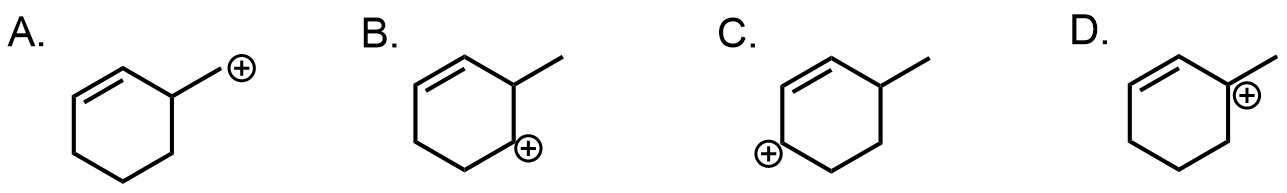
\includegraphics[scale=0.38, valign=c]{./Figure/2021/2021_4_1.png}
    \item 与Lucas试剂反应，体系立刻变浑浊的是
    \begin{tasks}(4)
        \task 正丁醇
        \task 酒精
        \task 苯甲醇
        \task 环己醇
    \end{tasks}
    \item 下列试剂中，三苯甲基醚不稳定的是
    \begin{tasks}(4)
        \task 碱
        \task Grignard试剂
        \task 烷基锂
        \task 酸
    \end{tasks}
    \item 下列化合物中，酸性最强的是
    
    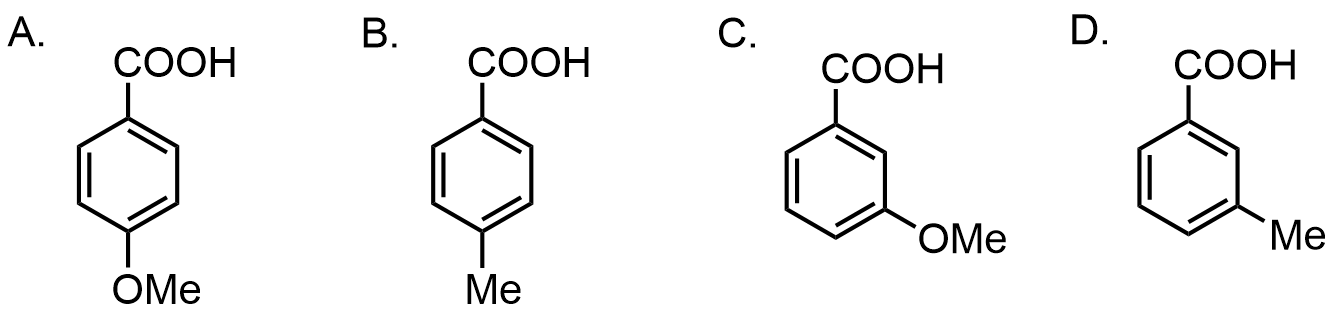
\includegraphics[scale=0.38, valign=c]{./Figure/2021/2021_4_4.png} 
    \item 不能与HCN反应的化合物是
    \begin{tasks}(4)
        \task 环戊酮
        \task 苯乙酮
        \task 苯甲醛
        \task 2-丁酮
    \end{tasks}
    \item 下列化合物中，不能发生溴仿反应的是
    \begin{tasks}(2)
        \task \ce{BrCH2COCH2CH3}
        \task \ce{PhCOCH3}
        \task \ce{CH3CH(OH)CH2CH3}
        \task \ce{PhCOC2H5}
    \end{tasks}
    \item 下列化合物具有芳香性的是
    
    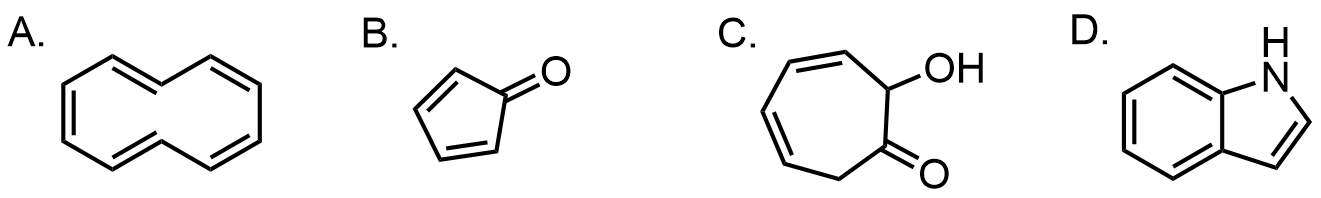
\includegraphics[scale=0.38, valign=c]{./Figure/2021/2021_4_7.png}
    \item 下列化合物中，不具有手性的分子是
    
    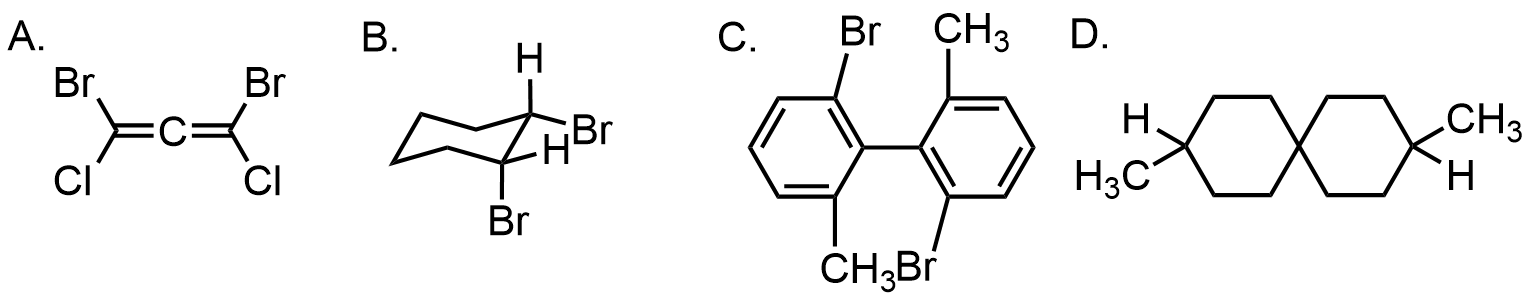
\includegraphics[scale=0.38, valign=c]{./Figure/2021/2021_4_8.png}
    \item 下列溶剂中，\ce{C2H5O-}的亲核性最强的是
    \begin{tasks}(4)
        \task 二甲亚砜
        \task 水
        \task 三氟乙酸
        \task 乙醇
    \end{tasks}
    \item 下列化合物与对甲基苯磺酰氯反应后既不溶于酸又不溶于碱的是
    \begin{tasks}(4)
        \task 乙胺
        \task 四氢吡咯
        \task 环戊胺
        \task 三乙胺
    \end{tasks}
    \item 下列亲双烯体中，[4+2]环加成反应活性最高的是
    
    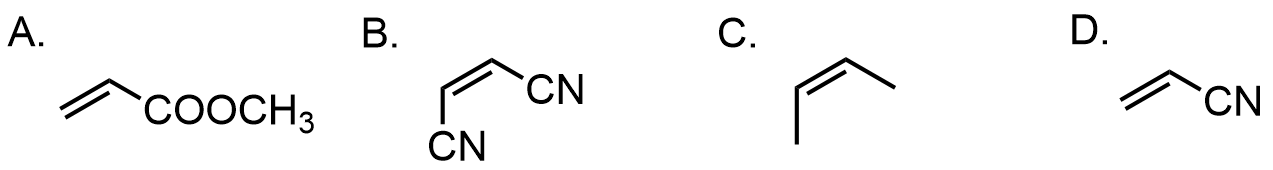
\includegraphics[scale=0.38, valign=c]{./Figure/2021/2021_4_11.png}
    \item 吡啶发生磺化反应时，磺酸基主要进入
    \begin{tasks}(4)
        \task $\alpha$位
        \task $\beta$位
        \task $\gamma$位
        \task $\alpha$位和$\gamma$位
    \end{tasks}
\end{enumerate}

\vspace{0.5cm}
\noindent\textbf{二、完成反应(32 pts.)}

\begin{enumerate}[label=\arabic*., itemsep=3ex]
    \item 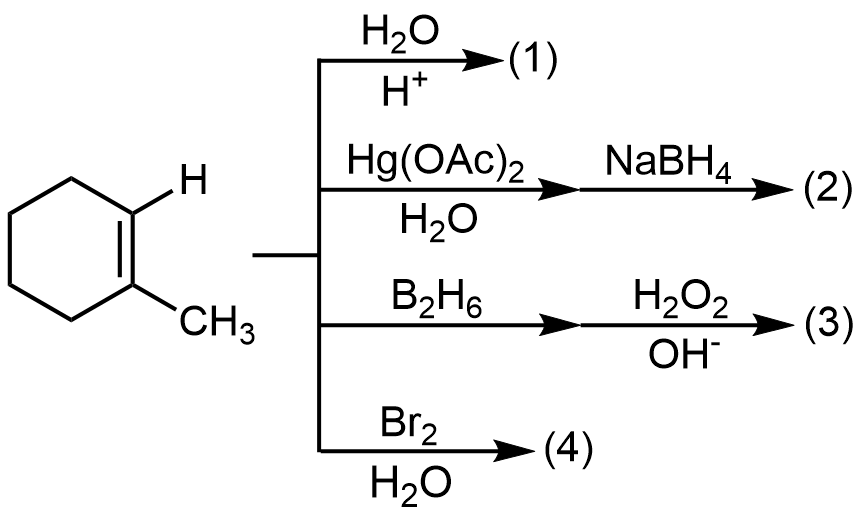
\includegraphics[scale=0.3, valign=c]{./Figure/2021/2021_1_1.png} 
    \item 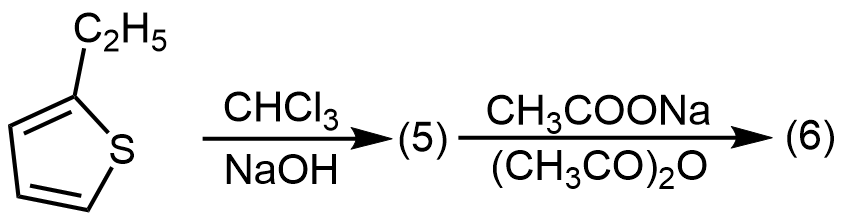
\includegraphics[scale=0.3, valign=c]{./Figure/2021/2021_1_2.png}
    \item 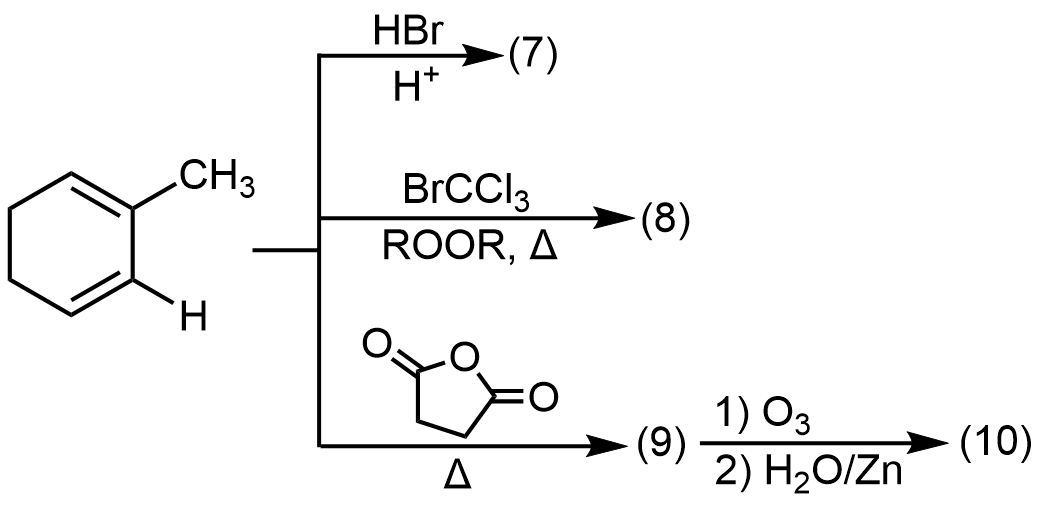
\includegraphics[scale=0.3, valign=c]{./Figure/2021/2021_1_3.png}
    \item 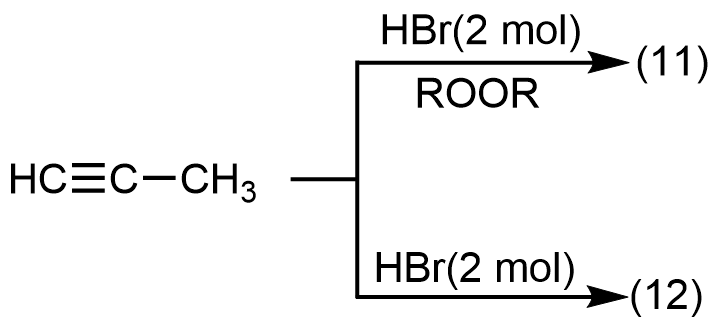
\includegraphics[scale=0.3, valign=c]{./Figure/2021/2021_1_4.png}
    \item 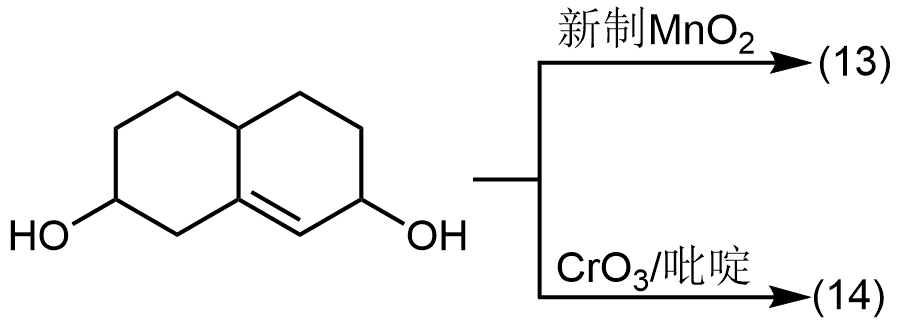
\includegraphics[scale=0.3, valign=c]{./Figure/2021/2021_1_5.png}
    \item 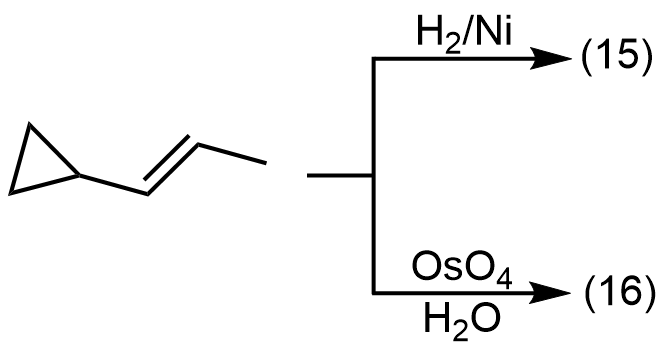
\includegraphics[scale=0.3, valign=c]{./Figure/2021/2021_1_6.png}
    \item 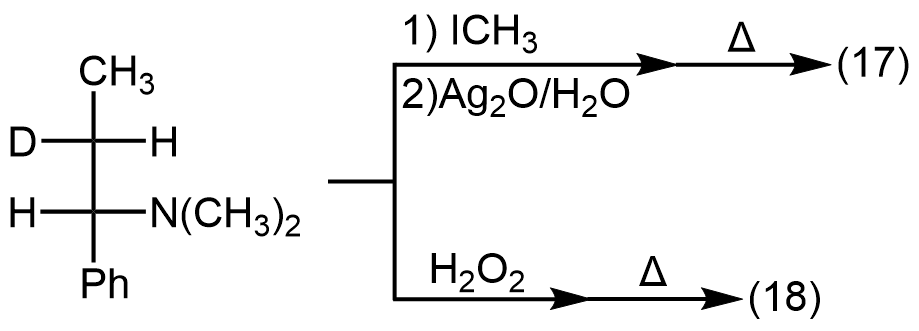
\includegraphics[scale=0.3, valign=c]{./Figure/2021/2021_1_7.png}
    \item 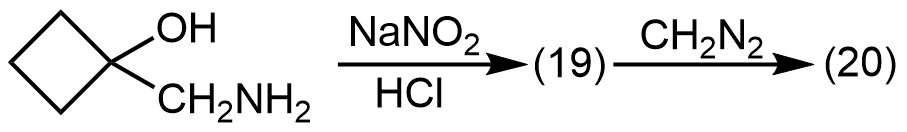
\includegraphics[scale=0.3, valign=c]{./Figure/2021/2021_1_8.png}
    \item 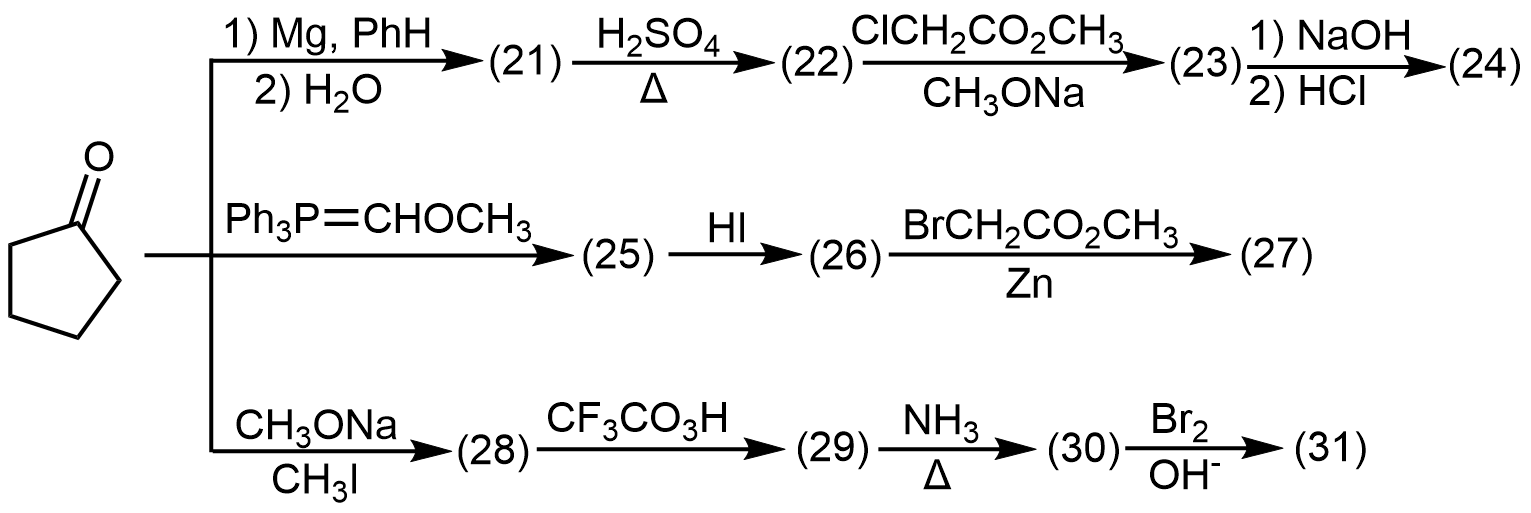
\includegraphics[scale=0.3, valign=c]{./Figure/2021/2021_1_9.png}
    \item 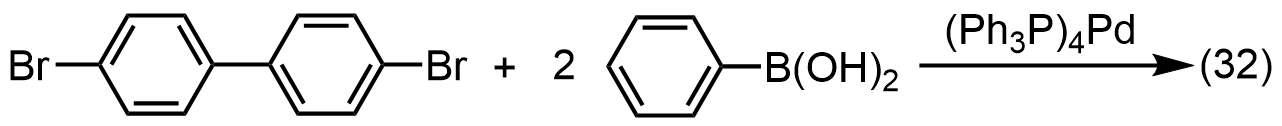
\includegraphics[scale=0.3, valign=c]{./Figure/2021/2021_1_10.png}

\end{enumerate}

\vspace{0.5cm}
\noindent\textbf{三、简答题(7 pts.)}

\begin{enumerate}[label=\arabic*., itemsep=3ex]
    \item 完成下列反应，给出其机理，并解释醛酮与羟胺反应生成肟需要用酸催化，却不能用强酸催化的原因。
    
    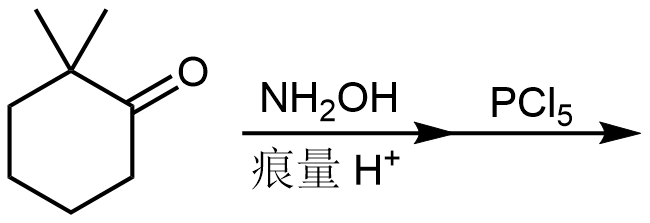
\includegraphics[scale=0.3, valign=c]{./Figure/2021/2021_5_1.png}
\end{enumerate}


\vspace{0.5cm}
\noindent\textbf{四、机理题(14 pts.)}

\begin{enumerate}[label=\arabic*., start=1, itemsep=1.5ex]
    \item 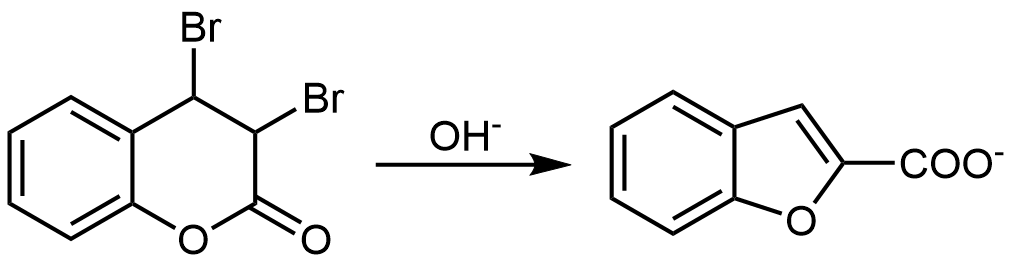
\includegraphics[scale=0.3, valign=c]{./Figure/2021/2021_2_1.png}
    \item 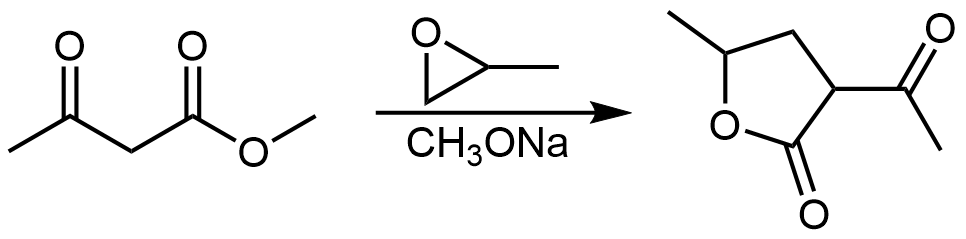
\includegraphics[scale=0.3, valign=c]{./Figure/2021/2021_2_2.png}

\end{enumerate}

\vspace{0.5cm}
\noindent\textbf{五、合成题(35 pts.)}

\begin{enumerate}[label=\arabic*., start=1, itemsep=1.5ex]
    \item 以丙炔为唯一有机原料合成\textbf{A}
    \item 以苯、小于等于4个碳的有机物合成\textbf{B}
    \item 以苯、小于等于2个碳的有机物合成\textbf{C}
    \item 以乙炔、小于等于3个碳的有机物合成\textbf{D}
    \item 以环己酮、小于等于3个碳的有机物合成\textbf{E}
    \begin{center}
        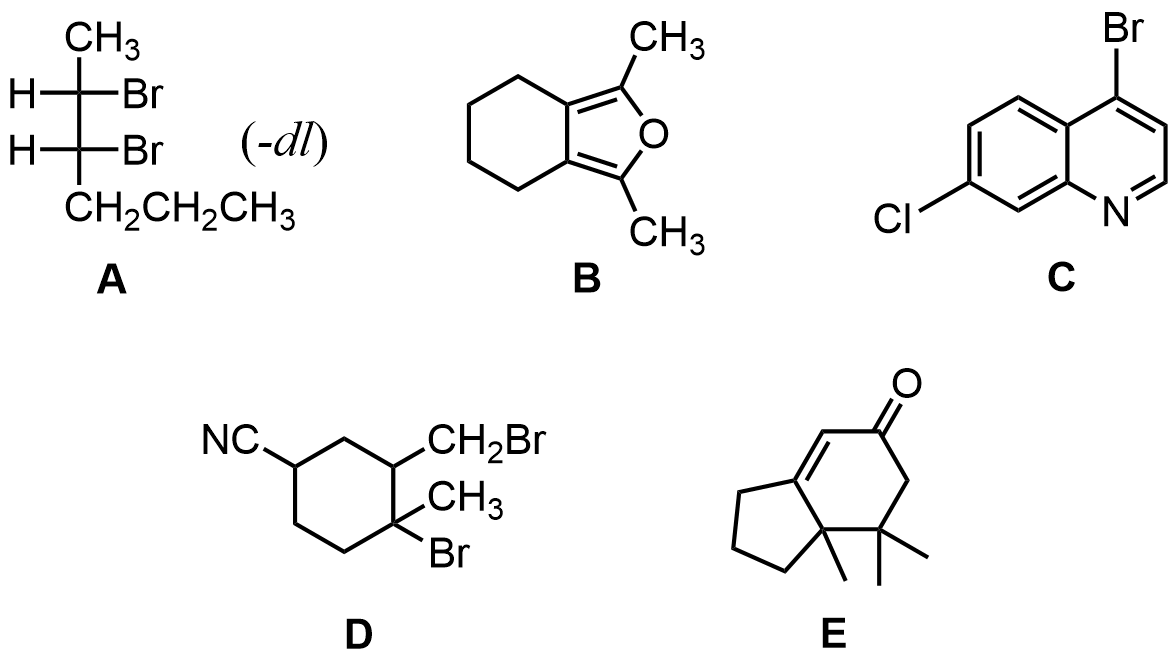
\includegraphics[scale=0.38]{./Figure/2021/2021_3.png}
    \end{center}
\end{enumerate}

\vspace{1cm}
\begin{center}
    {\Large \textbf{分析化学部分(共50分)}}
\end{center}


\vspace{0.5cm}
\noindent\textbf{六、简答题(20 pts.)}

\begin{enumerate}[label=\arabic*., itemsep=1.5ex]
    \item 用最小刻度为$0.01\,\text{g}$的台秤称取约$5\,\text{g}$的物品，最多可记录多少位有效数字？如用来测定土壤水分，要求称量的相对误差不大于$0.2\%$，至少应称取土壤试样多少克？
    \item 写出下列溶液的质子条件式：
    \begin{enumerate}[label=(\arabic*), noitemsep, topsep=0pt, partopsep=0pt]
        \item $\ce{NH4HCO3}$水溶液质子条件式。
        \item $\ce{NaOH}$和$\ce{NaAc}$混合水溶液的质子条件式（假定$\ce{NaOH}$在水溶液中全部离解，其浓度为$c_b$）。
        \item $\ce{H2NCH2COOH}$水溶液的质子条件式。
        \item $\ce{HAc-NaAc}$缓冲溶液的质子条件式（假定$\ce{HAc}$在缓冲溶液中浓度为$c_a$，$\ce{NaAc}$在缓冲溶液中浓度为$c_b$）。
    \end{enumerate}
    \item 若配制$\text{EDTA}$溶液的水中含有少量$\ce{Pb^{2+},Ca^{2+}}$，今在$\text{pH}\ 5\sim6$用纯锌为基准物标定其浓度。(1)测定$\ce{Al^{3+}}$（$\text{pH}5\sim6$，以$\ce{Zn^{2+}}$标准溶液返滴定过量的$\text{EDTA}$），其结果会怎样；(2)测定$\ce{Ca^{2+}}$其结果会怎样。（指偏高、偏低或无影响）
    \item 已知在$1\,\text{mol/L}\ \ce{HCl}$中，$\varphi^\ominus_{\ce{Fe^{3+}/Fe^{2+}}}=0.68\,\text{V}$；$\varphi^\ominus_{\ce{Sn^{4+}/Sn^{2+}}}=0.14\,\text{V}$，问以$\ce{Fe^{3+}}$滴定$\ce{Sn^{2+}}$至$99.9\%$、$100\%$、$100.1\%$时的电位分别为多少？
    \item 请简要回答为什么莫尔(Mohr)法适用的酸度范围是$\text{pH}=6.5-10.5$？
\end{enumerate}

\vspace{0.5cm}
\noindent\textbf{七、计算题(30 pts.)}

\begin{enumerate}[label=\arabic*., itemsep=1.5ex]
    \item 以$0.1000\,\text{mol/L}\ \ce{NaOH}$溶液滴定$0.2000\,\text{mol/L}\ \ce{HA}$和$0.2000\,\text{mol/L}\ \ce{HB}$的混合溶液。求：(1)判断是否能选择性滴定$\ce{HA}$，并计算滴定至化学计量点时体系的$\text{pH}$值；(2)若终点时$\text{pH}$值比化学计量点时高$0.5$个$\text{pH}$单位，终点误差是多少？
    
    [已知：$\ce{HA}$的$K_a=10^{-3.74}$，$\ce{HB}$的$K_a=10^{-9.26}$]
    \item 在$\text{pH}=5.0$时，以二甲酚橙作指示剂用$2.000\times10^{-2}\,\text{mol/L}\ \text{EDTA}$滴定浓度皆为$2.000\times10^{-2}\,\text{mol/L}$的$\ce{Pb^{2+}}$、$\ce{Zn^{2+}}$、$\ce{Ca^{2+}}$混合液中的$\ce{Pb^{2+}}$，用邻二氮菲(phen)掩蔽$\ce{Zn^{2+}}$，已知终点时phen游离浓度为$10^{-2.0}\,\text{mol/L}$，(1)问$\ce{Zn^{2+}}$被掩蔽的效果；(2)计算终点误差（忽略加掩蔽剂后的体积变化）。
    
    [已知：$\lg K_{\ce{PbY}}=18.0$，$\lg K_{\ce{ZnY}}=16.5$，$\lg K_{\ce{CaY}}=10.7$，$\ce{Zn-phen}$络合物的$\lg\beta_3=17.6$，$\text{pH}=5.0$时$\text{pPb}_\text{ep}$(二甲酚橙)$=7.0$、$\lg\alpha_{Y(\text{H})}=6.6$]
    \item 计算$\ce{Ag2S}$在$\text{pH}=9.0$的$\ce{NH3-NH4Cl}$缓冲溶液（$[\ce{NH3}]=0.10\,\text{mol/L}$），$\ce{S^{2-}}$总浓度为$0.10\,\text{mol/L}$溶液中的溶解度。
    
    [$\ce{H2S}$：$K_{a1}=1.3\times10^{-7}$，$K_{a2}=7.1\times10^{-15}$；$\ce{Ag^+-NH3}$络合物$\lg\beta_1,\lg\beta_2$依次为$3.4,7.4$；$K_{\text{sp}}(\ce{Ag2S})=2.0\times10^{-50}$]
\end{enumerate}